\documentclass[]{article}
\usepackage[a4paper, total={15cm,23cm}]{geometry}
\usepackage{fancyhdr}
\usepackage{graphicx}
\usepackage{amsmath}
\usepackage{amssymb}
\usepackage{xcolor}
\usepackage{tikz}
\usepackage{verbatim}
\usepackage{tcolorbox}
\usepackage{textcomp}
\usepackage{xcomment}
\usepackage{xstring}
\usepackage{array}
%opening
\title{PH 221 Week 3}
\author{Benjamin Bauml}
\date{Spring 2024}
\pagestyle{fancy}
\rhead{PH 221}
\chead{Spring 2024}
\lhead{Week 3}

% Version 2024-02-21
% Changes
% 2024-02-21 Added xstring package to enable smooth implementation of new \ModePage command.
% For Assignment, leave Purpose as 1. For Worksheet, set to 2. For Student Solution, set to 3. For Teacher Solution, set to 4.
\newcommand{\Purpose}{2}

\newcommand{\Exclusion}{0}
\newcommand{\PageTurn}{0}
\newcommand{\GrayProb}{0}
\newcommand{\Tipsy}{0}

% Assignment
\if\Purpose1
\renewcommand{\Exclusion}{1}
\fi
% Worksheet
\if\Purpose2
\renewcommand{\Exclusion}{1}
\renewcommand{\PageTurn}{1}
\fi
% Student Solution
\if\Purpose3
\renewcommand{\PageTurn}{1}
\renewcommand{\GrayProb}{1}
\fi
% Teaching Copy
\if\Purpose4
\renewcommand{\PageTurn}{1}
\renewcommand{\GrayProb}{1}
\renewcommand{\Tipsy}{1}
\fi

\if\Exclusion1
\xcomment{Title,Problem,ProblemSub,PassFig}
\fi

\def \NewQ {0}
\def \PForce {0}
\newcommand{\MaybePage}[1]{
	\def \PForce {#1}
	\if\PForce1
		\newpage
	\else
		\if\NewQ0
		\gdef \NewQ {\PageTurn}
		\else
		\newpage
		\fi
	\fi
}

\newcommand{\ModePage}[1]{
	\IfSubStr{#1}{\Purpose}{\newpage}{}
}

\newenvironment{Problem}[2][0]{%The first argument is optional, and if it is set to 1, the \newpage will be forced.
\MaybePage{#1}
\section*{#2}
\if\GrayProb1
\begin{tcolorbox}[colback=lightgray,colframe=lightgray,sharp corners,boxsep=1pt,left=0pt,right=0pt,top=0pt,bottom=0pt,after skip=2pt]
\else
\begin{tcolorbox}[colback=white,colframe=white,sharp corners,boxsep=1pt,left=0pt,right=0pt,top=0pt,bottom=0pt,after skip=2pt]
\fi
}{
\end{tcolorbox}\noindent
}

\newenvironment{ProblemSub}[1][0]{%The argument is optional, and if a string of numbers is entered into it, it will force a \newpage in any \Purpose that shows up in the string. For example, "13" would lead to the newpage being forced in modes 1 and 3.
\ModePage{#1}
\if\GrayProb1
\begin{tcolorbox}[colback=lightgray,colframe=lightgray,sharp corners,boxsep=1pt,left=0pt,right=0pt,top=0pt,bottom=0pt,after skip=2pt]
\else
\begin{tcolorbox}[colback=white,colframe=white,sharp corners,boxsep=1pt,left=0pt,right=0pt,top=0pt,bottom=0pt,after skip=2pt]
\fi
}{
\end{tcolorbox}\noindent
}

\newenvironment{PassFig}{\begin{figure}[h]}{\end{figure}}

\newcommand{\TeachingTips}[1]{
\if\Tipsy1
\begin{tcolorbox}[colback=lightgray,colframe=black]
#1
\end{tcolorbox}
\fi
}

\newenvironment{Title}{\maketitle}{}

\begin{document}
\begin{Title}
\end{Title}

\begin{Problem}{Activity}
	You are standing in a large building, and there is a single window right up by the ceiling. This window opens on an alleyway, and the building on the other side has an open window below the level of your building's window. You want to launch something from your building into the other, right through the center of each window. You know the heights of the windows and the width of the alley, so what do you need to do to throw it correctly?
\end{Problem}
\begin{ProblemSub}
	(1) Draw a physical representation of the situation. On this drawing, indicate the height of the center of the first window $ h_{1} $, the height of center of the second window $ h_{2} $, the width of the alley $ w $, the initial velocity $ \vec{v}_{0} $, the launch angle $ \theta $, and your distance to the wall of the first window $ d $. Add a coordinate system (indicate the directions of $ +x $ and $ +y $), and indicate the direction of gravitational acceleration $ \vec{g} $. What are your unknowns?
\end{ProblemSub}
\begin{figure}[h]
	\centering
	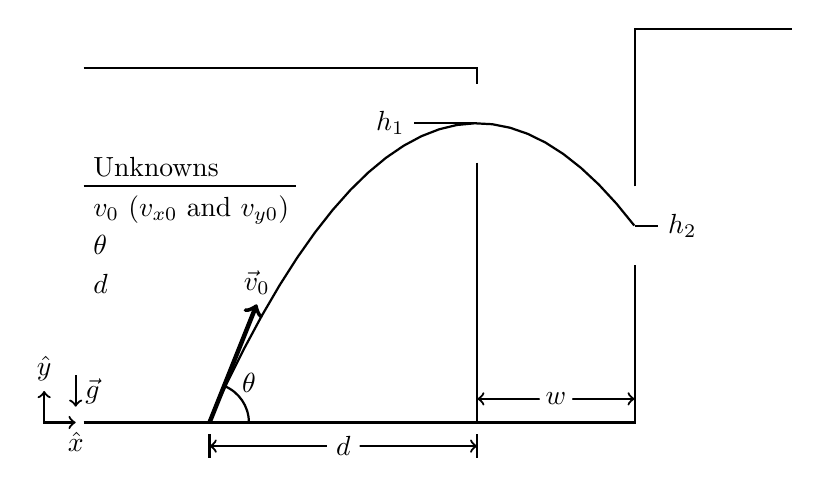
\begin{tikzpicture}
		\draw[thick] (-4,0) -- (3,0) -- (3,2);
		\draw[thick, <->] (1,0.3) -- (3,0.3);
		\filldraw[white] (2,0.3) circle (0.2);
		\node at (2,0.3) {$w$};
		\draw[thick] (3,2.5) -- (3.3,2.5);
		\node[anchor=west] at (3.3,2.5) {$h_{2}$};
		\draw[thick] (3,3) -- (3,5) -- (5,5);
		\draw[thick] (-4,4.5) -- (1,4.5) -- (1,4.3);
		\draw[thick] (1,3.8) -- (0.2,3.8);
		\node[anchor=east] at (0.2,3.8) {$h_{1}$};
		\draw[thick] (1,3.3) -- (1,0);
		\draw[thick] (1,-0.15) -- (1,-0.45);
		\draw[thick, domain = -1.95:1.14, variable = \x]  plot ({1.75*\x+1},{-\x*\x+3.8});
		\draw[thick] (-2.4,-0.15) -- (-2.4,-0.45);
		\draw[thick, <->] (-2.4,-0.3) -- (1,-0.3);
		\filldraw[white] (-0.7,-0.3) circle (0.2);
		\node at (-0.7,-0.3) {$d$};
		\draw[ultra thick, ->] (-2.4,0) -- (-1.8,1.5);
		\node[anchor=south] at (-1.8,1.5) {$\vec{v}_{0}$};
		\draw[thick] (-1.9,0) arc (0:68.2:0.5);
		\node at (-1.9,0.5) {$\theta$};
		\node[anchor=south west] at (-4,3) {Unknowns};
		\draw[thick] (-4,3) -- (-1.3,3);
		\node[anchor=north west]  at (-4,3) {$v_{0}$ ($v_{x0}$ and $v_{y0}$)};
		\node[anchor=north west]  at (-4,2.5) {$\theta$};
		\node[anchor=north west]  at (-4,2) {$d$};
		\draw[thick, <->] (-4.5,0.4) -- (-4.5,0) -- (-4.1,0);
		\node[anchor=south] at (-4.5,0.4) {$\hat{y}$};
		\node[anchor=north] at (-4.1,0) {$\hat{x}$};
		\draw[thick, ->] (-4.1,0.6) -- (-4.1,0.2);
		\node[anchor=west] at (-4.1,0.4) {$\vec{g}$};
	\end{tikzpicture}
\end{figure}
\begin{ProblemSub}
	(2) Since the window is right by the ceiling, you cannot arc your projectile too high. Suppose for simplicity that you want it to reach its maximum height right as it goes through the first window. What must its initial velocity be in the $ y $ direction for this to happen?
\end{ProblemSub}
We know the final $ y $-velocity at the peak of motion will be zero, and we know the object will have traveled $ \Delta y = h_{1} $, so we can use the kinematics equation which does not involve time of flight:
\begin{equation}
	\begin{split}
		v_{y}^{2} & = v_{y0}^{2} + 2a_{y}\Delta y \\
		0 & = v_{y0}^{2} - 2gh_{1} \\
		v_{y0} & = \sqrt{2gh_{1}}.
	\end{split}
\end{equation}
\begin{ProblemSub}[34]
	(3) Exiting the first window, the object only has velocity in the $ x $ direction. How long does it take to fall to the height of the second window? How fast must it be going to cross the alley in this time and enter the second window?
\end{ProblemSub}
The horizontal velocity has no impact on the vertical motion of the object. It begins at $ y_{i} = h_{1} $ and free-falls to $ y_{f} = h_{2} $, starting from $ v_{yi} = 0 $. The change in position kinematics equation gives us
\begin{equation}
	\begin{split}
		y_{f} & = y_{i} + v_{yi}\Delta t + \frac{a_{y}}{2}(\Delta t)^{2} \\
		h_{2} & = h_{1} + 0 - \frac{g}{2} (\Delta t_{h_{1}\to h_{2}})^{2} \\
		h_{1}-h_{2} & = \frac{g}{2} (\Delta t_{h_{1}\to h_{2}})^{2} \\
		\Delta t_{h_{1}\to h_{2}} & = \sqrt{\frac{2(h_{1}-h_{2})}{g}}.
	\end{split}
\end{equation}
The velocity $ v_{x} $ does not change during flight, as there is no horizontal component to acceleration. As such, it must be that the object has total velocity $ \vec{v} = v_{x0}\hat{\imath} $ as it leaves the first window. It must travel across $ \Delta x = w $ over time $ \Delta t_{h_{1}\to h_{2}} $ to enter the other window, which means
\begin{equation}
	\begin{split}
		\Delta x & = v_{x0}\Delta t + \frac{a_{x}}{2}(\Delta t)^{2} \\
		w & = v_{x0}\Delta t_{h_{1}\to h_{2}} + 0 \\
		v_{x0} & = \frac{w}{\Delta t_{h_{1}\to h_{2}}} = w \sqrt{\frac{g}{2(h_{1}-h_{2})}}.
	\end{split}
\end{equation}
\begin{ProblemSub}
	(4) Given the horizontal and vertical components of initial velocity, how far back from the first window do you have to stand to get the object through it?
\end{ProblemSub}
The link between the $ x $ and $ y $ kinematics equations is $ \Delta t $, which is shared between them. As such, we must find the time it takes for the object to reach $ \Delta y = h_{1} $, then we must find how far $ \Delta x = d $ it travels horizontally in that time. We begin with
\begin{equation}
	\begin{split}
		\Delta y & = v_{y0}\Delta t + \frac{a}{2}(\Delta t)^{2} \\
		0 & = \Delta y - v_{y0}\Delta t - \frac{a}{2}(\Delta t)^{2} \\
		& = h_{1} - v_{y0}\Delta t + \frac{g}{2}(\Delta t)^{2}.
	\end{split}
\end{equation}
Now we have a form to which we can apply the quadratic formula, which gives
\begin{equation}
	\begin{split}
		\Delta t & = \frac{-(-v_{y0}) \pm \sqrt{(-v_{y0})^{2} - 4(g/2)(h_{1})}}{2(g/2)} \\
		& = \frac{v_{y0} \pm \sqrt{v_{y0}^{2} - 2gh_{1}}}{g}.
	\end{split}
\end{equation}
Inserting our expression from part (2), we get
\begin{equation}
	\begin{split}
		\Delta t & = \frac{\sqrt{2gh_{1}} \pm \sqrt{2gh_{1} - 2gh_{1}}}{g} \\
		& = \frac{\sqrt{2gh_{1}}}{g} \\
		& = \sqrt{\frac{2h_{1}}{g}}.
	\end{split}
\end{equation}
Without acceleration, we know that $ \Delta x = v_{x0} \Delta t $. With our new expression for $ \Delta t $, plus our expression for $ v_{x0} $ from part (3), we find
\begin{equation}
	d = \Delta x = w\sqrt{\frac{g}{2(h_{1}-h_{2})}}\sqrt{\frac{2h_{1}}{g}} = w \sqrt{\frac{h_{1}}{h_{1}-h_{2}}}.
\end{equation}
\begin{ProblemSub}
	(5) Given the components of initial velocity, what is the magnitude of initial velocity? At what angle with respect to the floor must the object be launched?
\end{ProblemSub}
The magnitude of velocity is simply the result of the Pythagorean theorem:
\begin{equation}
	v_{0} = \sqrt{v_{x0}^{2}+v_{y0}^{2}} = \sqrt{\frac{w^{2}g}{2(h_{1}-h_{2})} + 2gh_{1}}.
\end{equation}
The angle requires an application of trigonometry. If $ v_{0} $ is the hypotenuse of a right triangle with legs $ v_{x0} $ and $ v_{y0} $, then the angle $ \theta $ is opposite $ v_{y0} $ and adjacent to $ v_{x0} $. This means
\begin{equation}
	\tan\theta = \frac{v_{y0}}{v_{x0}}.
\end{equation}
Taking the inverse tangent of both sides will recover $ \theta $. A good sensemaking technique with recovering angles in this way is to think about the relative sizes of the triangle's legs. If $ v_{y0} > v_{x0} $, then we are guaranteed that $ \theta > 45^{\circ} $.
\end{document}